\documentclass[]{article}
\usepackage[style=numeric,backend=biber,sorting=none]{biblatex}
\usepackage{graphicx}
\usepackage{float}
\usepackage{pgfplots}
\addbibresource{references.bib}

% Title Page
\title{Financial Analysis Report}
\author{Mark Paveszka}


\begin{document}
\maketitle

\newpage

\begin{abstract}
\end{abstract}

\newpage

\tableofcontents

\newpage

\section{Introduction}
\paragraph{}
As a result of modern technology, the way things are done is very different compared how it was twenty years ago. Since then everything has been speeding up, including a key area of society, namely: education. In the past fifteen to twenty years several businesses emerged to make education better and easier for both students and teachers. These businesses usually try to create software artefacts to improve some aspect of the broader field. Such software artefacts are innovative learning tools and learning management systems (LMS). One of the most well-known companies in the education technology sector is Blackboard \cite{Blackboard_UK}. They provide several applications to improve the quality of teaching in higher education, business and governmental institutes. They are mostly known for Blackboard Learn \cite{Blackboard_Learn}, which is one of the most popular learning management systems currently available on the market based on data collected by Client Stat \cite{VLE-Data} and analysed by Edutechinca \cite{VLE-2020-IMG}. The aggregation of this data is shown in Figures \ref{fig:LMS-2020} and \ref{fig:LMS-2020-6-year} which depict the market share of the most popular learning management systems in four different regions. For the purpose of this analysis only the data regarding the UK will be considered. The main competitors to Blackboard are Moodle, Canvas and Brightspace. 

\begin{figure}
    \centering
    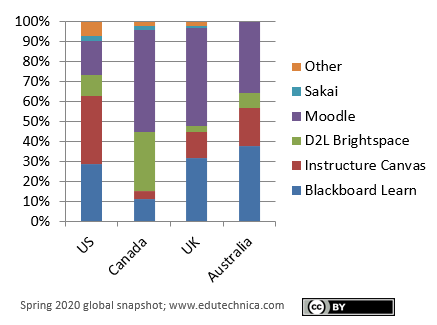
\includegraphics[width =\linewidth]{lms-vle-2020.png}
    \caption{LMS market share in 2020. \cite{VLE-2020-IMG}}
    \label{fig:LMS-2020}
\end{figure}

\begin{figure}
    \centering
    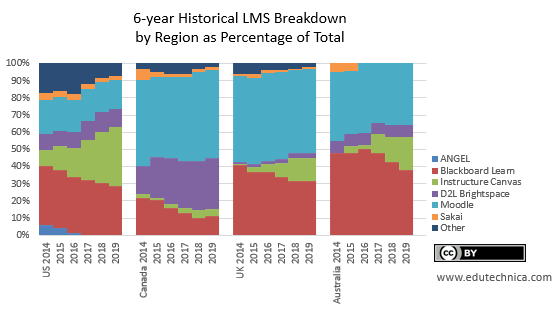
\includegraphics[width =1.2\linewidth]{lms-vle-2020-y5.png}
    \caption{6-year historical LMS data by region. \cite{VLE-2020-IMG}}
    \label{fig:LMS-2020-6-year}
\end{figure}

\paragraph{}
To obtain some data about these companies an online tool, namely Software Advice \cite{Software-Advice} was used. This tool allowed for comparisons between the companies, which provided further insight about them. The result showed that Blackboard, Canvas and Brightspace compete in the same price range, while Moodle is cheaper to use. After examining different sources it is clear that Blackboard is not a cheap software to use \cite{Blackboard-v-Moodle}, however it provides a wide variety of features for the institutions that opt to use their system.

\paragraph{}
In 2017 the education technology sector in the UK worth around £170m \cite{Government-Strategy}. This number by 2021 is expected grow to to £3.4bn which shows that there is a lot of potential in this sector. However it is worth noting that the LMS market is part of the education technology sector and even though there will be growth it might not be that significant. Also globally there is not much change \cite{VLE-2020-IMG} in the usage of these systems compared to previous years based on Edutechnica's analysis. Globally speaking there is going to be a massive growth \cite{Markets-and-Markets} even when looking at what is projected for Europe (Figure \ref{fig:Markets-LMS}). However it is worth noting that market size of Europe will only be a small portion of the global market.

\begin{figure}
    \centering
    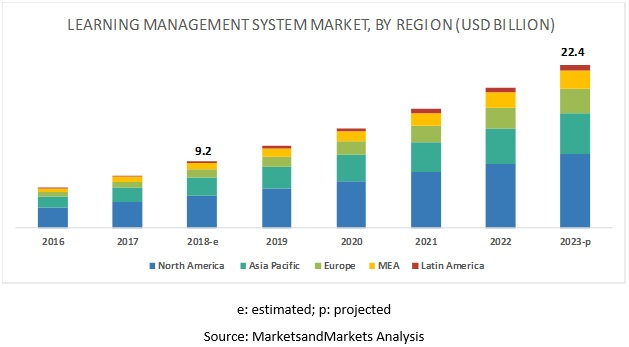
\includegraphics[width =1.2\linewidth]{learning-management-systems-market5.jpg}
    \caption{Market growth projection. \cite{Markets-and-Markets}}
    \label{fig:Markets-LMS}
\end{figure}

\section{Financial Analysis}
\paragraph{}
In order to determine how successful Blackboard is, its financial situation needs to be examined. The following information was obtained by using FAME which is a financial database about UK based companies. To perform the analysis ratios will be used, which can be found in Table \ref{tab:Ratios-BB}. It is worth noting that Blackboard is a private company, so it is harder to find some information about it, as it does not have to publish financial statements. In Blackboard's FAME report \cite{FAME-Blackboard} the latest data entry was created in 2018. This data suggests that for the past two years the shareholder funds were decreasing somewhat. However before that this number jumped from £860k to £65m which indicates a large scale investment into the company. In 2017 the ROCE (Return on Capital Employed) ratio dropped below 0. The -14.24\% ROCE is due to the fact that the company generated a massive loss (PBT) of £-8m. This troubling trend continued in 2018, however the situations was a bit better as the ROCE value was -1.65\% which is still not negative, however it is significantly better than the 2017 one. These issues could be explained by events that happened to the company during these years. First of all Moodle ended their partnership with Blackboard \cite{Moodle-breaks-up-with-Blackboard}, which have lowered the trust in their customers. The extent this event affected the company was quite severe as they have lost their very first customers (Cornell University) in the same year \cite{Cornell-leaves-BB}. These two events combined could have easily resulted in loss of trust from other customers. It is worth noting that throughout this period, and even today Blackboard is receiving a lot of complaints for not having user friendly graphical interfaces \cite{BB-Reviews}, which could also suggest that customers were not satisfied about its products.

\paragraph{}
By taking a closer look at the Return on Shareholders Capital \ref{tab:Ratios-BB}, several conclusions can be drawn. First, the ratio values for 2018, 2017 and 2016 are the same as the ROCE values. This indicates that the total capital employed is the same as the shareholders' funds. This means that in the years mentioned, Blackboard did not have any short term loans. Secondly, the fact that this ratio was negative in the past means that Blackboard was not really popular for new investors. This is further reinforced by the fact that the Interest Cover ratio was also negative which means that Blackboard was unable to pay proper interest payments. However before 2017 this ratio was quite good, as it was 32.38\%. It must be kept in mind that Blackboard UK only had short term group loans from their parent company in the United States. Since this loan was provided by the parent company not being able to pay interest was probably not such a severe issue as if they had to pay for banks and other companies.


%TABLE
\begin{table}
\centering
\begin{tabular}{||c | c | c | c | c||} 
\hline
Ratio & 2018 & 2017 & 2016 & 2015 \\ [0.5ex] 
\hline\hline
ROCE \% & -1.65 & -14.24 & 3.39 & 96.31 \\ 
\hline
Return on shareholders capital \% & -1.65 & -14.24 & 3.39 & 99.87 \\ 
\hline
Gearing \% & 32.26 & 25.32 & 27.70 & n.s. \\ 
\hline
Interest Cover (x) & -7.52 & n.s. & 32.38 & 15.77 \\ 
\hline
Current Ratio (x) & 0.97 & 0.64 & 0.79 & 0.36	 \\ 
\hline
Quick Ratio (x) & 0.97 & 0.64 & 0.79 & 0.36 \\ 
\hline
Profit Margin \% & -2.77 & -27.08 & 5.95 & 6.33 \\ 
\hline
\end{tabular}
\caption{Ratios for Blackboard (UK) Limited from 2018 to 2015 \cite{FAME-Blackboard}}
\label{tab:Ratios-BB}
\end{table}


\paragraph{}
By looking at the quick ratio and the current ratio of the past years it is clear that they are equal. This means that there is no significant inventory that Blackboard has, which is expected since they are a selling software artefacts instead. The quick ratio measures the liquidity of a company and since there is no change to the current ratio in this case, Blackboard is probably not very good in this sense. Comparing the values of both the quick and the current ratio to the education services average values \cite{Ready-Ratios-Education} visible in Table \ref{tab:Ratios-EDSec} we can conclude several things. First that in all the years examined the current ratio remained significantly under the industry average which means that indicates higher risk of distress \cite{Investopedia-Current}. Moreover the ratio always stayed below 0 which indicates that if all of the short term obligations were due at the same time, the company would not have enough capital on hand to pay them back. The quick ratio followed the trend of remaining below average from 2015 to 2017. However in 2018 the value of the ratio (0.97) surpassed the industry average (0.86). Since the current and quick ratios were the same, they measure the same aspect of the company. Everything said for the current ratio is also true for the quick ratio. This fact also reinforces the fact that investors were not drawn to the company as they have feared that it won't be able to pay back its liabilities towards them.

\paragraph{}
By taking a look at the gearing ratio it can be concluded that there is definitely more shareholder funding in the company than long and short term loans. The gearing ratio values can be considered acceptable and good between 25\% and 50\% \cite{Investopedia-Gearing}. Based on this information Blackboard's gearing ratios in the years between 2018 and 2016 were in the acceptable range, however it was always on the lower side, rather than the upper. Even though the gearing ratio was in the optimal range, the fact that the company did not generate profits in its last two operating years can mean that the debtors would not want to give loans as it is questionable if the company can actually repay the existing debts. Also the fact there is no inventory based on the quick and current ratios, which means that there is no way for the company to quickly gain money to repay liabilities. This probably even further reduces the debtors will to provide loans for the company.


%TABLE
\begin{table}
\centering
\begin{tabular}{||c | c | c | c | c||} 
\hline
Ratio & 2018 & 2017 & 2016 & 2015 \\ [0.5ex] 
\hline\hline
Current Ratio (x) & 1.05 & 1.50 & 1.53 & 1.34 \\ 
\hline
Quick Ratio (x) & 0.86 & 1.23 & 1.24 & 1.34 \\ 
\hline
\end{tabular}
\caption{Average ratio values for Education Services sector from 2018 to 2015 \cite{Ready-Ratios-Education}}
\label{tab:Ratios-EDSec}
\end{table}


\paragraph{}
Based on the profit margins (PBT / Turnover) Blackboard was doing well during the 2015 and 2016 (Figure \ref{fig:BB-Profit-Margin}), as they respective profit margins were both above 5\%. However, there is a massive drop in 2017, which is due to the fact that the company generated an £8m loss. It is also clear that regardless off this loss Blackboard is getting better, since their profit margin in 2018 was almost 10 times better than the year before. But even with that increase in performance they still generated loss, as their profit margin shows. 

\begin{figure}
    \centering
    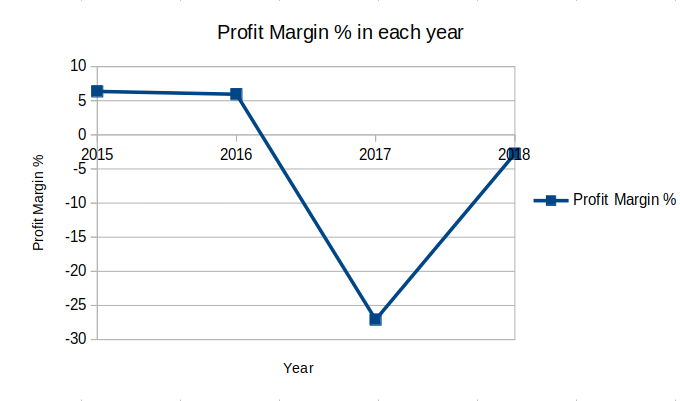
\includegraphics[width =1.2\linewidth]{profit margin.png}
    \caption{Blackboard's historical profit margin data based on FAME \cite{FAME-Blackboard}}
    \label{fig:BB-Profit-Margin}
\end{figure}

%TABLE
\begin{table}
\centering
\begin{tabular}{||c | c | c | c||} 
\hline
Ratio & 2018 & 2017 & 2015 \\ [0.5ex] 
\hline\hline
Current Ratio (x) & 1.08 & 1.09 & 1.07 \\ 
\hline
Quick Ratio (x) & 1.08 & 1.09 & 1.07 \\ 
\hline
Gearing \% & 243.33 & 2.90 & 238.34 \\ 
\hline
\end{tabular}
\caption{Ratio values for D2L Europe Limited from 2015, 2017 and 2018 \cite{FAME-D2L}}
\label{tab:Ratios-D2L}
\end{table}


\paragraph{}
To get a full view on Blackboard's financial status it is crucial to analyse other companies as well in the same sector. The companies behind Blackboard Learn's competitors will be analysed. These companies are Instructure Global Limited \cite{FAME-Instructure} and D2L Europe Limited \cite{FAME-D2L}. The latter company did not release an in-depth report, therefore only some ratios are available. Only the quick, current and gearing ratios are available for years 2015, 2017 and 2018, which can be seen in Table \ref{tab:Ratios-D2L}. Since this is also a company that produces software artefacts it was expected that the quick and current ratios will be equal. Based on the data, this company was in a better financial situation than Blackboard UK in the past couple of years as they had capital on hand to pay off their current liabilities in each year. On Figure \ref{fig:LMS-2020-6-year} it is visible that D2L's product is slowly gaining popularity in the UK, which could explain this phenomenon. In terms of the gearing ratio D2L had major fluctuations as it was either really high, or really low. This could happen due to the fact that the company took loans. This  is still in the 300\% tolerance range, which means even when the ratio was high and the investors considered it as risky it was still a manageable risk.

%TABLE
\begin{table}
\centering
\begin{tabular}{||c | c | c | c | c||} 
\hline
Ratio & 2018 & 2017 & 2016 & 2015 \\ [0.5ex] 
\hline\hline
ROCE \% & 120.57 & 401.96 & 498.92 & -285.99 \\ 
\hline
Interest Cover (x) & -7.39 & -23.35 & -35.49 & n.s. \\ 
\hline
Current Ratio (x) & 0.87 & 0.81 & 0.51 & 0.75 \\ 
\hline
Quick Ratio (x) & 0.87 & 0.81 & 0.51 & 0.75 \\ 
\hline
Profit Margin \% & -15.34 & -53.64 & n.s. & n.s.\\ 
\hline
\end{tabular}
\caption{Ratio values for Instructure Global Limited from 2015, 2017 and 2018 \cite{FAME-Instructure}}
\label{tab:Ratios-Instructure}
\end{table}

\paragraph{}
Insturcture Global Limited is the company that is creating the Canvas LMS. Currently in the industry the market share of this product is rapidly increasing, which is visible on Figure \ref{fig:LMS-2020-6-year}. This process is reflected in the ratios as well (Table \ref{tab:Ratios-Instructure}. Since 2016 Instructure's ROCE ratio is quite high, over 100\% which means that the return is much greater than the capital employed for operating. The fact that this platform is gaining popularity can also explain why Blackboard hs been struggling with finances in the past years. In terms of interest cover rates Blackboard and Instructure is very close to each other, however while Blackboard's values are decreasing, Instructure's are increasing. By comparing the rest of the data it can be said that Instructure is currently in a better situation as it is more desirable for investors than Blackboard, mostly because the latter lost a lot of market in the past couple of years. 

\section{Change to the product}

\paragraph{}
Even though Blackboard is still one of the market leaders in Learning Management Systems, the company is slowly losing its market shares, as visible in Figure \ref{fig:LMS-2020-6-year}. Recently it lost the most popular LMS title in the United States \cite{Canvas-overtakes-BB}, and it is just a matter of time till they lose it in the UK as well. 

\paragraph{}
One of the biggest complaints about Blackboard Learn is it's clunky user interface. There are several complaints on both Trust Radius \cite{BB-Reviews} and on other platforms such as Capterra \cite{Capterra-BB-Reviews}, that criticise and place the UI into disadvantages and negative point about the website. These reviews say that Blackboard could be very useful as it offers a lot of features and integrate a lot of outside services such as Turnitin, that could make processes more efficient, however the bad user interface which is full of bugs makes the product's user experience very unpleasant. This unpleasant experience is leading to existing customers changing to different and more modern Learning Management Systems with more user-friendly UIs such as Canvas or Moodle \cite{BB-Alternatives}.

\paragraph{}
For this reasons the suggested change is the improvement of the User Interface design, on scientific principles, keeping the users in the center of focus. Such improvements could mean that customers who like the functionality provided by Blackboard, but are not satisfied with its interface could probably be convinced to reconsider and return to the product. Moreover, a good user interface is indispensable nowadays, as without it, web based applications cannot thrive and be popular \cite{UI-Advantages}. This would certainly add value to the company, as with a user-friendly interface implementation new customers could be gained, and the trust lost during the years could be restored. As said in the \textit{Introduction} the LMS market is likely to grow in general by 2025, which means that there are many new potential customers. However, it is key that Blackboard understands that the new interface has to be centered around the user experience. There is more behind a bad web design than being ugly. It can undesired effects on the company that owns it, such as hurting the established brand, and creating an even worse customer experience \cite{bad-design-why}, each of which can lead to further loss of customers. Therefore it is crucial, that during development of a new UI, this mistake is avoided by keeping the in mind the user-centered design paradigms. 


\paragraph{}
However, changing the user interface is not an easy task. This process can be long and costly, especially if Blackboard thrives to design for UX. Designing for user experience requires a lot of steps as research, development, testing and evaluation. It si very important to involve UX specialist into the process who can execute this steps with great efficiency \cite{UX-30000}. Designing for UX is based on scientific methods, which Blackboard might not be too familiar with. Performing the necessary research with the right people, and testing with a representative set of users is quite costly. In short term, for Blackboard to design a new interface is a definitive expenditure, however in terms of the future, they will definitely profit from it, in case of a user experience centered design outcome. 

\paragraph{}
It must be kept in mind all times that while creating a new user interface, the old one must be supported as well, which means that bugs need to be fixed. This is necessary, since if Blackboard drops all support for its current interface, they will lose more customers, which is will impact their ability to finance research and development of a new UX focused design. Moreover there might be additional costs involved. Newer front-end frameworks most of the times require new server side technologies. In order to build a modern framework, that will be operational for several years, most of the times newer systems needs to be developed. In best case scenario Blackboard was continuously upgrading their system, and therefore there are no legacy systems involved. In this case creating a good user interface could take up to 4-6 months at least \cite{UX-30000}. After this the implementation of this interface could also take up to 4-5 months \cite{Webredesign-adv} which means that in total in optimal conditions there is at least a year needed for this new interface. This of course means that additional staff has to be hired for the duration of this project. Costs for such designs could vary, but in general they are not cheap \cite{UX-cost}. On average the UX designers usually take around \$200 per hour or work, and in a large scale project like this they might as for more. This means that if Blackboard employs two UX designers that could cost them around \$500k plus the salaries for the developers who will implement the created design, which is a significant expense 

\paragraph{}
The worst case scenario is when Blackboard is running some of its services from legacy systems. In this case they would need extra developers to recreate their LMS with newer technologies. This would of course cost a significant amount of money, as both the work needed to be done and the time required to do implement the necessary changes would be much greater than the one in the optimal scenario. These changes would include the complete migration of their system to new server side frameworks, meanwhile still supporting the current version of their product, both in terms of UI and server side issues. Additionally, there is a cost for retraining existing customer support staff so they would be able to handle customer issues. However, changing to a new system can reduce future upkeep costs as people who are managing the legacy systems would not be needed anymore. Also newer systems tend to be more efficient and faster, which will further reduce costs of maintenance. 

\paragraph{}
Examples show that such actions can seriously impact future revenue and finances. Such an example is the Business2Community website which redesigned its web interface in 2018 \cite{Redesign-case-study}. After they have went through with the process their website traffic was increased by a 100\%. Even though Blackboard probably will not have such numbers as their customers are mostly institutions, there will be improvements, as both students and teachers will be content with their products.


\begin{table}
\centering
\begin{tabular}{||c | c | c ||} 
\hline
 & 2018 & 2017 \\ [0.5ex] 
\hline\hline
Turnover & 33,855,313 & 30,173,418 \\ 
\hline
Cost of Sales & (2,462,847) & (2,402,189) \\ 
\hline
Administrative Expenses & (32,744,970) & (36,215,530) \\ 
\hline
Staff Cost & (7,924,936) & (8,847,579) \\ 
\hline
\end{tabular}
\caption{Main expenses and incomes in £ of Blackboard UK in 2017 and 2018 \cite{FAME-Blackboard}}
\label{tab:Statement-BB}
\end{table}

\section{Cutting Costs}
\paragraph{}
In order to cut costs for Blackboard, the financial statements of it have to be examined. For the purpose of these decision the report of 2018 will be used which is available on Blackboard's FAME profile \cite{FAME-Blackboard}. Upon examining the the financial report it is clear that Blackboard was doing better in 2018 than 2017, as they had a bigger turnover by £3m, which is visible on Table \ref{tab:Statement-BB}. By far the biggest expenses of the company are the administrative expenses. The total sum of these expenses is barely lower than the turnover itself, which means that any other expenses that the company might generate potentially results in losses. As it is seen in the table, the cost of sales is an additional £2.4m which when added to the administrative expenses immediately generate loss. Therefore the best way to cut cost at this company is at the administrative expenses level. 

\paragraph{}
Before diving into the possibilities what cost can be reduced at the company, the concept of administrative expenses has to be cleared. Every expense that are not directly tied to main operations such as manufacturing or sales is considered to be a part of administrative expenses. Such expenses include the salaries for senior management, property rent and utilities \cite{Investopedia-Administrative}. Blackboard (UK) Limited's main office is located in London \cite{GOV-BB}, very close to the City of London where the main financial district is. Based on Blackboard's financial report they do not own any properties, which means that the main office they work in is being rented by them. In this area the average office space costs £69.5/square foot \cite{Statista-Rent-London}. 

\paragraph{}
Based on the report provided by FAME, Blackboard in 2018 had 63 employees. This number than can be used in an online tool named Zoopla \cite{Zoopla} to calculate average office space size needed for Blackboard. With this the option standard work space was selected which means 95 square feet / person annually. Based on this the space needed for the company is 5985 square feet, which is quite a lot. This multiplied with the average office space price, the average yearly rent price of their office is calculated, which is around £417k. It is clear that the rent they are paying is quite high, which definitely could be reduced, if the office was moved from the heart of London to the outer districts. For example in Croydon, London which 40 minutes from the current office the rental prices are less than a third to what Blackboard is paying currently, based on information obtained from Zoopla \cite{Zoopla-search}. This means that they could pay £65k annually which is 85\% saving on rent. Unfortunately in general administrative expenses are hard to reduce, because they are mostly fixed, however with careful decentralization and delegation this could be further reduced, since oversight expenses will be less \cite{Investopedia-Administrative-reduce}. 

\paragraph{}
One thing that can be reduced is the salary of the executives in the company. Typically speaking executives salaries are quite high \cite{Executives}, which means that some additional funds could be gained by reducing them. According to PayScale \cite{Executives-avg-salary} the average executive salary in the UK is between £110k to £115k per year. For the sake of this calculation an average of £110k will be used. According to Blackboard currently in the UK there are 10 executives that are working \cite{leaders-BB}, which puts the total amount of executive salaries around £1.1m. Since this is not a very large sum compared to their expenses, and usually in a company executives are not expected to give up their salaries, this amount should only be reduced by 10\% till the financial status of the company stabilises. This would mean that in total there would be around an extra £110k available for the company, which when compared to the turnover is a really small amount.

\paragraph{}
However, as visible in Table \ref{tab:Statement-BB}, Blackboard also has significant expenses on staff. As previously mentioned in 2018 they had 63 employees working for them. In 2017 the staff cost was almost a £1m larger than in 2018. This is due to the fact that in 2017 Blackboard employed 71 people, which could suggest that Blackboard was reducing the number of employees. However if the broader picture is viewed, it is clear that Blackboard was always working with around 60 people, which suggests in 2017 they have hired extra people for one-year long tasks. In 2018 therefore the company employed around the amount of people as they did in previous years. In order to further cut costs downsizing is needed. Based on the data available from FAME, on average the employees are payed £125k which is in total almost £8m. This means if the company reduces the number of employees by 4, it could gain additional £500k available funds. However this downsizing must be carefully done, since the company would not want to lose its best skilled workers, as they are needed for growth. Therefore Blackboard should reduce employees in positions which do not require high skills to do. Instead of hiring people to do these jobs, Blackboard could outsource it to another company. This would be beneficial, as they will not have invest into training and salaries \cite{forbes-outsourcing}. 

\paragraph{}
In total these measures could reduce Blackboard's expenditures quite significantly, with a total of £962k. This amount would almost cover the company's loss in 2018. Organic growth is a slow process, it requires time and patience from Blackboard. It is also worth noting that in general Blackboard was doing almost 10 times as better in 2018 than in 2017, which suggests that it will continue to stabilise in the future. This and the cost reductions together should be able to prepare Blackboard for organic growth.

\newpage





\printbibliography{}

\end{document}          
